\lecture{9.1}{Non-Binary and Continuous Treatments}
\label{lec:9-1}

\subsection{Review of Point Exposures}

For a point exposure, the observed data for one individual are
\[
  O=(W,A,Y),
\]
where $W$ denotes pre-treatment covariates, $A$ denotes treatment or exposure,
and $Y$ denotes the outcome. Earlier chapters focused mainly on binary
treatments, but the counterfactual notation is not limited to binary $A$. For
any exposure value $a$ in the support of $A$, write
\[
  \Ya{a}
\]
for the outcome that would be observed if the exposure were set to $a$.

\subsection{Binary ATE}

When $A\in\{0,1\}$, the average treatment effect is
\[
  \ATE=\E(\Yone)-\E(\Yzero).
\]
Under consistency, conditional exchangeability, and positivity,
\[
  \E\{\Ya{a}\}=\E\{\E(Y\given A=a,W)\},
\]
so
\[
  \ATE
  =
  \E\{\E(Y\given A=1,W)-\E(Y\given A=0,W)\}.
\]
This is a contrast between two points on a counterfactual response surface.

\subsection{Continuous Exposures}

If $A$ is continuous, there is no single treated-versus-untreated comparison.
Instead, the target is usually the entire causal response curve
\[
  \mu(a)=\E\{\Ya{a}\},\qquad a\in\mathcal{A},
\]
or a contrast between two exposure levels,
\[
  \mu(a)-\mu(a'),\qquad
  \frac{\mu(a)}{\mu(a')},\qquad
  \dd{\mu(a)}{a}.
\]
The derivative is meaningful only when the dose-response curve is sufficiently
smooth and the intervention ``increase exposure infinitesimally'' is scientifically
well-defined.

\subsection{Dose-Response Curves}

\begin{definition}[Causal dose-response curve]
For an exposure $A$ with support $\mathcal{A}$, the causal dose-response curve is
the function
\[
  a\mapsto \mu(a)=\E\{\Ya{a}\}.
\]
It maps each intervention level $a$ to the mean outcome that would be observed
if every member of the target population were assigned that level.
\end{definition}

\begin{figure}[H]
\centering
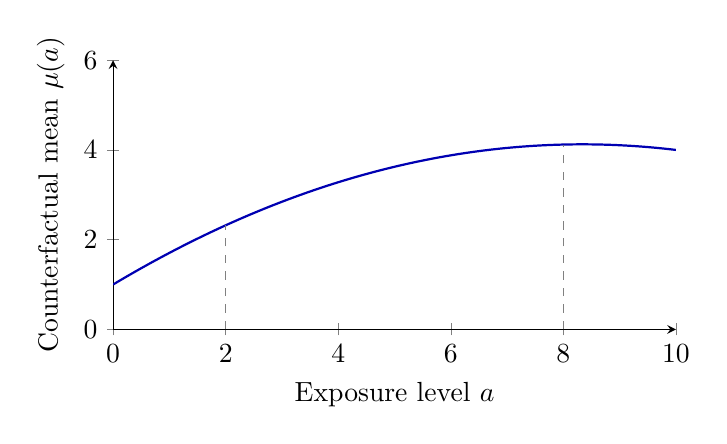
\begin{tikzpicture}
\begin{axis}[
  width=.72\textwidth,
  height=5cm,
  xlabel={Exposure level $a$},
  ylabel={Counterfactual mean $\mu(a)$},
  xmin=0,xmax=10,ymin=0,ymax=6,
  axis lines=left,
  samples=100
]
\addplot[blue!70!black, thick, domain=0:10] {1 + .75*x - .045*x^2};
\addplot[dashed, gray] coordinates {(2,0) (2,2.32)};
\addplot[dashed, gray] coordinates {(8,0) (8,4.12)};
\end{axis}
\end{tikzpicture}
\caption{A dose-response curve is a collection of counterfactual means indexed by exposure level.}
\label{fig:ch9-dose-response}
\end{figure}

\subsection{Identification Assumptions for Non-Binary Treatments}

\begin{assumptionbox}
For every $a\in\mathcal{A}$:
\[
  \text{Consistency:}\qquad A=a\Rightarrow Y=\Ya{a}.
\]
\[
  \text{Conditional exchangeability:}\qquad \Ya{a}\ci A\given W.
\]
\[
  \text{Positivity:}\qquad f_{A\given W}(a\given w)>0
  \text{ whenever } f_W(w)>0
  \text{ and } a \text{ is targeted}.
\]
\end{assumptionbox}

Under these assumptions,
\[
\begin{aligned}
  \E\{\Ya{a}\}
  &=\E\left[\E\{\Ya{a}\given W\}\right]\\
  &=\E\left[\E\{\Ya{a}\given A=a,W\}\right]\\
  &=\E\left[\E(Y\given A=a,W)\right].
\end{aligned}
\]
The first equality is the tower rule, the second uses conditional
exchangeability, and the third uses consistency.

\begin{identificationbox}
The dose-response curve is identified by
\[
  \mu(a)=\E\{\E(Y\given A=a,W)\}.
\]
For discrete non-binary $A$, this formula is evaluated at each exposure category.
For continuous $A$, it is evaluated across exposure values in the target support.
\end{identificationbox}

\subsection{Positivity With Continuous Treatments}

Continuous-treatment positivity is stronger than it first appears. Since
$\Prob(A=a\given W=w)=0$ for any exact point $a$, positivity is stated in terms
of conditional densities. The data must contain enough individuals near exposure
level $a$ for each covariate profile $w$ being standardized over.

Practical positivity problems arise when:
\begin{itemize}
  \item some exposure values occur only in narrow covariate strata;
  \item the target curve includes doses outside the observed range;
  \item the conditional density $f_{A\given W}(a\given w)$ is very small;
  \item scientific interventions at some levels are not meaningful or safe.
\end{itemize}

\begin{keyidea}
For non-binary treatments, the causal estimand is usually a response curve or a
contrast along that curve. Identification still uses consistency,
exchangeability, and positivity, but positivity becomes a support condition over
the exposure distribution.
\end{keyidea}
